\documentclass[11pt,a4paper]{article}
\usepackage{ucs}
\usepackage[T1]{fontenc}
\usepackage[utf8x]{inputenc}
\usepackage[german]{babel}
\usepackage{amsmath}
\usepackage{amsfonts}
\usepackage{amssymb}
\usepackage{graphicx}
\usepackage{shadethm}
\usepackage{caption}
\usepackage{tikz} 
\usepackage{ziffer}
\usepackage{units}
\usepackage{multirow}
\usepackage{subfigure}
\usepackage{hyperref}
\usepackage{cleveref}
\usepackage{braket}
\usepackage[procnames]{listings} %quellcode einbinden
 \usepackage{color}	% syntaxhighlighting
 \definecolor{keywords}{RGB}{255,0,90}
 \definecolor{comments}{RGB}{0,0,113}
 \definecolor{red}{RGB}{160,0,0}
 \definecolor{green}{RGB}{0,150,0}
 \lstset{language=Python, 
         basicstyle=\ttfamily\small, 
         keywordstyle=\color{keywords},
         commentstyle=\color{comments},
         stringstyle=\color{red},
         showstringspaces=false,
         identifierstyle=\color{green},
         procnamekeys={def,class}}

\newcommand{\minipanf}{\begin{minipage}{\linewidth}}
\newcommand{\minipend}{\end{minipage}}
\newcommand{\abs}[1]{\ensuremath{\left\vert#1\right\vert}}

\begin{document}

\begin{titlepage}
\newcommand{\HRule}{\rule{\linewidth}{0.5mm}} % Defines a new command for the horizontal lines, change thickness here

\center % Center everything on the page
 
%----------------------------------------------------------------------------------------
%	HEADING SECTIONS
%----------------------------------------------------------------------------------------

\textsc{\LARGE TU Dresden}\\[1.5cm] % Name of your university/college
\textsc{\Large Fortgeschrittenenpraktikum}\\[0.5cm] % Major heading such as course name
\textsc{\Large Praktikumsbericht}\\[0.5cm] % Major heading such as course name

%----------------------------------------------------------------------------------------
%	TITLE SECTION
%----------------------------------------------------------------------------------------

\HRule \\[0.7cm]
{ \huge \bfseries Lebensdauer von Myonen}\\[0.4cm] % Title of your document
\HRule \\[1.5cm]
 
%----------------------------------------------------------------------------------------
%	AUTHOR SECTION
%----------------------------------------------------------------------------------------

\begin{minipage}{0.4\textwidth}
\begin{flushleft} \large
\emph{Autoren:}\\
Toni \textsc{Ehmcke}\\
Christian \textsc{Siegel}
\end{flushleft}
\end{minipage}
~
\begin{minipage}{0.4\textwidth}
\begin{flushright} \large
\emph{Betreuer:} \\
Maximilian \textsc{Hils} % Supervisor's Name
\end{flushright}
\end{minipage}\\[4cm]

%----------------------------------------------------------------------------------------
%	DATE SECTION
%----------------------------------------------------------------------------------------

{\large Dresden, \today}\\
\vspace{5mm}
{\large Durchführungstag, 08. Januar 2016}\\

\vfill 

\end{titlepage} 	% Titelseite

\tableofcontents
\newpage 

\section{Einführung}

	\subsection{Entstehung von Myonen}
	\textit{Myonen} $\mu{\pm}$ lassen sich im heute gängigen Standardmodell der Teilchenphysik zur zweiten Generation der elektrisch geladenen Leptonen zuordnen. Sie sind mit $m_\mu = 105,658\ \unit{MeV = 206,768\ m_e}$\cite{pdg} die schweren Pendants zum Elektron.\\
	Im folgenden Versuch werden Myonen aus der kosmischen Höhenstrahlung, welche zu 85\% aus hochenergetischen Protonen besteht, untersucht. Bei Zusammenstößen dieser Protonen mit Atomkernen in der Erdatmosphäre entstehen die geladenen $\pi^\pm$-Mesonen Reaktionen niedrigster Ordnung sind:
		\begin{align*}
			&p + p \longrightarrow p + n + \pi^+\\
			&p + n \longrightarrow p + p + \pi-
		\end{align*}
	Diese Mesonen zerfallen nach etwa $2,6\cdot10^{-8}\ \unit{s}$ über die schwache Wechselwirkung. Der mit einem Anteil von 99,988\% dominierende Zerfallskanal endet in einem Myon und einem zugehörigen Neutrino und kann mit folgender Zerfallsgleichung und dem Feynmandiagramm in Abbildung \ref{fig:pionzerfall} beschrieben werden:
		\begin{align*}
			&\pi^+ \longrightarrow \mu^+ + \nu_\mu\\
			&\pi^- \longrightarrow \mu^- + \bar{\nu}_\mu\\
		\end{align*}
		\begin{figure}[hp]
					\centering
					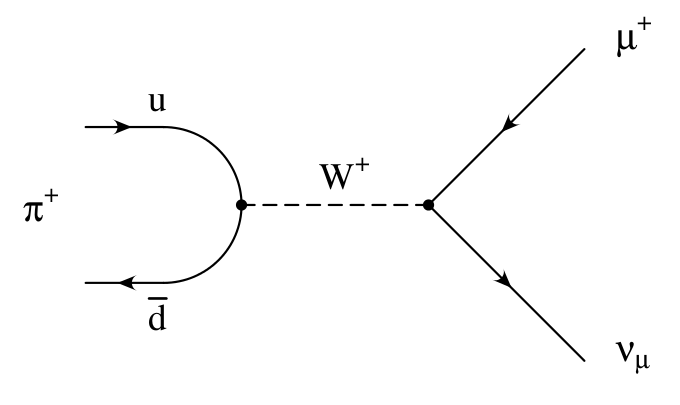
\includegraphics[width = 0.7\linewidth]{pic/pionzerfall.png}
					\caption{Feynman-Diagramm des Antimyonenzerfalls.}
					\label{fig:pionzerfall}
		\end{figure}
		
	\subsection{Zerfall von Myonen}
	Da das Myon ein sehr schweres Teilchen ist, zerfällt es nach einer sehr kurzen Zeit von:\cite{PA}\\
		\begin{equation} \label{eq:lit}
			\tau_\mu = (2,19703 \pm 0,00004)\ \unit{\mu s}
		\end{equation}
	mit nahezu 100\% über den schwachen Zerfall, der mit Hilfe der Reaktionsgleichungen (\ref{eq:mup}) und (\ref{eq:mum}) und zugehörigem Feynmangraph (nur niedrigste Ordnung) in Abbildung \ref{fig:myonzerfall} beschrieben werden kann.\\
	
		\begin{align}
			&\mu^+ \longrightarrow e^+ + \nu_e + \bar{\nu}_\mu 		\label{eq:mup}\\
			&\mu^- \longrightarrow e^- + \bar{\nu}_e + \nu_\mu 		\label{eq:mum}
		\end{align}
		\begin{figure}[hp]
			\centering
			\scalebox{0.5}[0.5]{
			\input{pic/myonzerfall.pdf_tex}
			}
			\caption{Feynman-Diagramm des Antimyonenzerfalls.}
			\label{fig:myonzerfall}
		\end{figure}
	\ \\
	Auch wenn die in Gleichung (\ref{eq:lit}) angegebene Lebensdauer sehr kurz erscheint, ist der Myonenfluss auf Meereshöhe mit $170\ \unit{Myonen/(m^2s)}$ sehr hoch. Dies lässt sich dadurch erklären, dass die oben angegebene Lebensdauer im Laborsystem der Beobachter auf der Erde angegeben ist. Da sich Myonen mit relativistischen Energien bewegen, besitzen sie in ihrem Ruhesystem eine \textit{zeitdilatierte Lebensdauer}, welche ausreicht, um an die Erdoberfläche zu gelangen. Selbst in der theoretischen Vorhersage der Lebensdauern mit Hilfe von \textit{Übergangsmatrixelementen} $\Gamma_{fi} = 1/\tau_{fi}$ (d.h. bei Übergang von Zustand $\ket{i}$ in $\ket{f}$) treten Terme auf, die nicht lorentzinvariant sind.
	
	\subsection{$\mu^-$-Einfang}
	Im Falle der negativ elektrisch geladenen Myonen $\mu^-$ existiert in Materie allerdings ein weiterer 'Zerfallskanal', der sogenannte $\mu^-$-Einfang, bei dem ein einfallendes Myon im Coulombfeld eines Atoms eingefangen wird, bis in den Grundzustand vordringt und anschließend vom Kern absorbiert wird. Dabei findet folgende Kernumwandlung(Abbildung \ref{fig:myoneinfang}) statt:
		\begin{equation*}
			\mu^- + p \longrightarrow  \nu_\mu + n 
		\end{equation*}
		
		\begin{figure}[ht]
			\centering
			\scalebox{1.}[1.]{
			\input{pic/myoneneinfang.pdf_tex}
			}
			\caption{Feynman-Diagramm des Myoneneinfangs.}
			\label{fig:myoneinfang}	
		\end{figure}
	\ \\
	Ist $\Gamma_z = 1/\tau_z$ die Partialbreite  des schwachen Zerfallskanals (\ref{eq:mum}) und $\Gamma_e=1/\tau_e$ die des $\mu^-$-Einfangs, ergibt sich die totale Breite des $\mu^-$-Zerfalls zu:
		\begin{align}
			&\Gamma_{\mu^-} = \Gamma_z + \Gamma_e\\
			&\tau_{\mu^-} = \left(\frac{1}{\tau_z} + \frac{1}{\tau_e}\right)^{-1} < \tau_{\mu^+}  
		\end{align}
	Im Praktikumsversuch werden die Myonen mit einer Kupferplatte eingefangen. Da der $\mu^-$-Einfang dafür sorgt, dass nach etwa $1\ \unit{\mu s}$ alle negativ geladenen Fermionen eingefangen worden, dominieren die $\mu^+$-Zerfälle die Messung. 
	
	\subsection{Messprinzip und Versuchsaufbau}
    \begin{figure}
        \centering 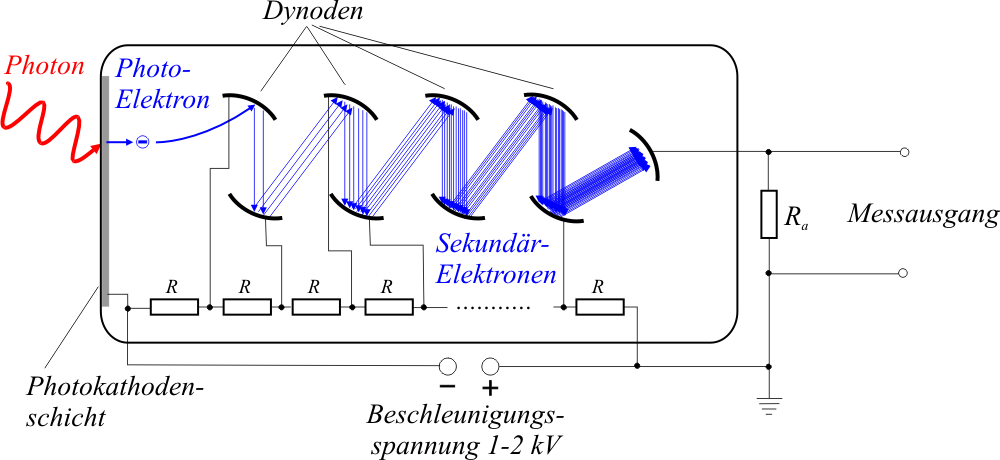
\includegraphics[scale=0.85]{pic/pm.png}
        \caption{\cite{pm} Skizze des Aufbaus eines PM}
    \end{figure}
	%TODO@Christian: Kurz beschreiben wie Szintillator und PM funktioniert + Versuchsaufbau (nur Messaufbau 1)			% Physikalischer Hintergrund
\section{Durchführung}
    \subsection{Vorversuche Gruppe B, LM1}
        Bevor mit dem Hauptversuch begonnen werden kann, müssen diverse Vorversuche durchgeführt werden, um die Versuchsparameter zu optimieren.
        \subsubsection{Aufnahme der Kennlinie von Photomultiplier 3 (PM3)}
            Als erstes soll nach Aufgabenstellung die Kennlinie des PM3 aufgenommen werden. Dafür muss zunächst die Messtechnik angeschlossen werden. In diesem Versuch wurde das Koinzidenzsignal (1·2·3) auf den Counter 1 und das einfache Signal 3 auf den Counter mit der Nummer 2 gelegt.\\
            Danach stellt man die Hochspannungen für die Multiplier 1 und 2 ($U_{1,HV}$ und $U_{2,HV}$) auf jeweils etwa $\unit[2400]{V}$ ein. Danach wird die Hochspannung für Photomultiplier 3 auf etwa $2100\unit{V}$ geregelt. Diese Gruppe erreichte für PM1 $U_{1,HV} = 2403\unit{V}$, für $U_{2,HV} = 2401\unit{V}$ und für $U_{3,HV} = 2099\unit{V}$. 
            Nun erfolgt die Evaluierung der Messdauer. Dafür muss zunächst über den relativen Fehler ermittelt werden, wie viele Counts gemessen werden sollen. 
            $$ \frac{\Delta N}{N} = N^{-\frac{1}{2}} \leq 3\unit{\%}$$
            Da die Counts poisson-verteilt sind, erhält man für $\Delta N = \sqrt{N}$. Die Zahl der zu messenden Ereignisse (Counts) ergibt sich über diese Rechnung zu 1112. Nun wählt man im Messprogramm die Option ab, die Messung nach einer bestimmten Zeit anzuhalten und misst solange, bis Counter 1 ungefähr den errechneten Wert erreicht, wobei zu beachten ist, dass der gemessene Wert größer ist, um den relativen Fehler unterhalb der $3\unit{\%}$ zu halten. Diese Gruppe hat für einen Counter-Wert von 1122 eine Messdauer $t_{Mess} = 117\unit{s}$ gemessen. Diese Zeit wird für die Aufnahme der Kennlinie benötigt.
            Für die Aufnahme der Kennlinie des PM3 wird die Spannung $U_{3,HV}$ in $50\unit{V}$-Schritten von $1800\unit{V}$ bis $2400\unit{V}$ variiert. Die Stufen werden $t_{Mess}$ lange gemessen. 
            \begin{figure}[htbp]
                \subfigure[Kennlinie des PM3 mit Signal $N_{1·2·3}$\label{n123}]{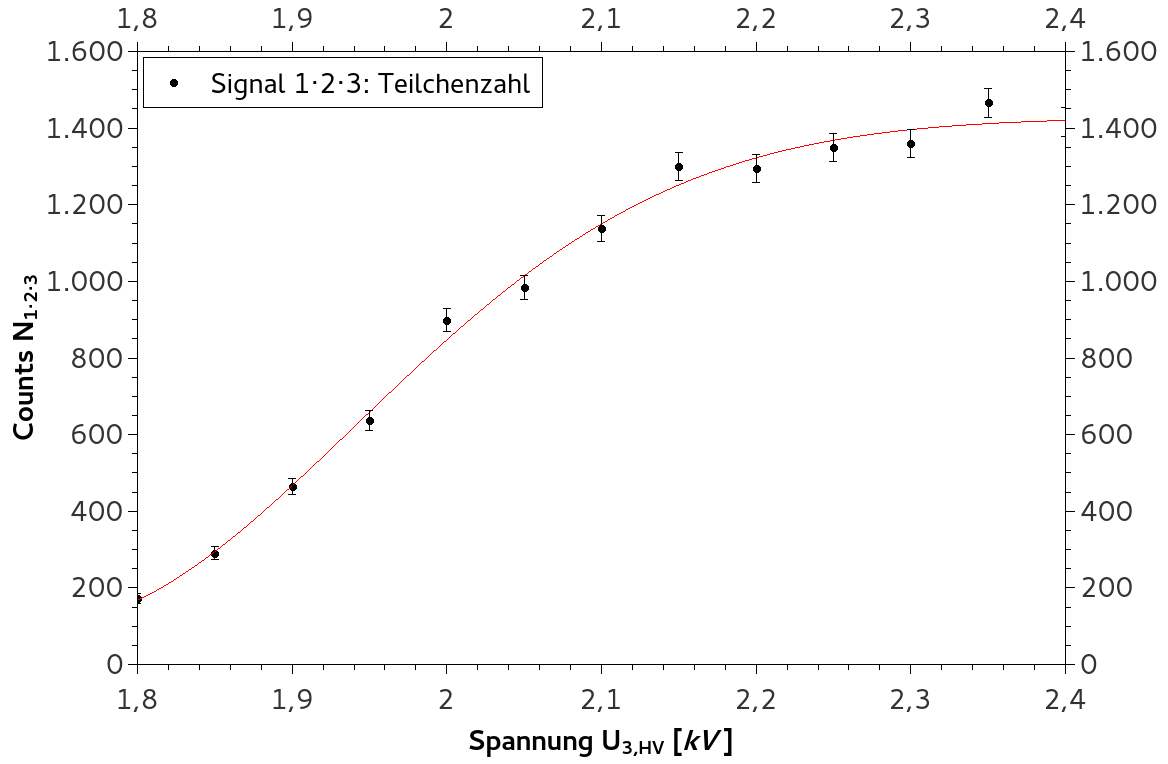
\includegraphics[scale=0.225]{pic/n123u3th}}
                \subfigure[Kennlinie des Signals $N_3$\label{n3}]{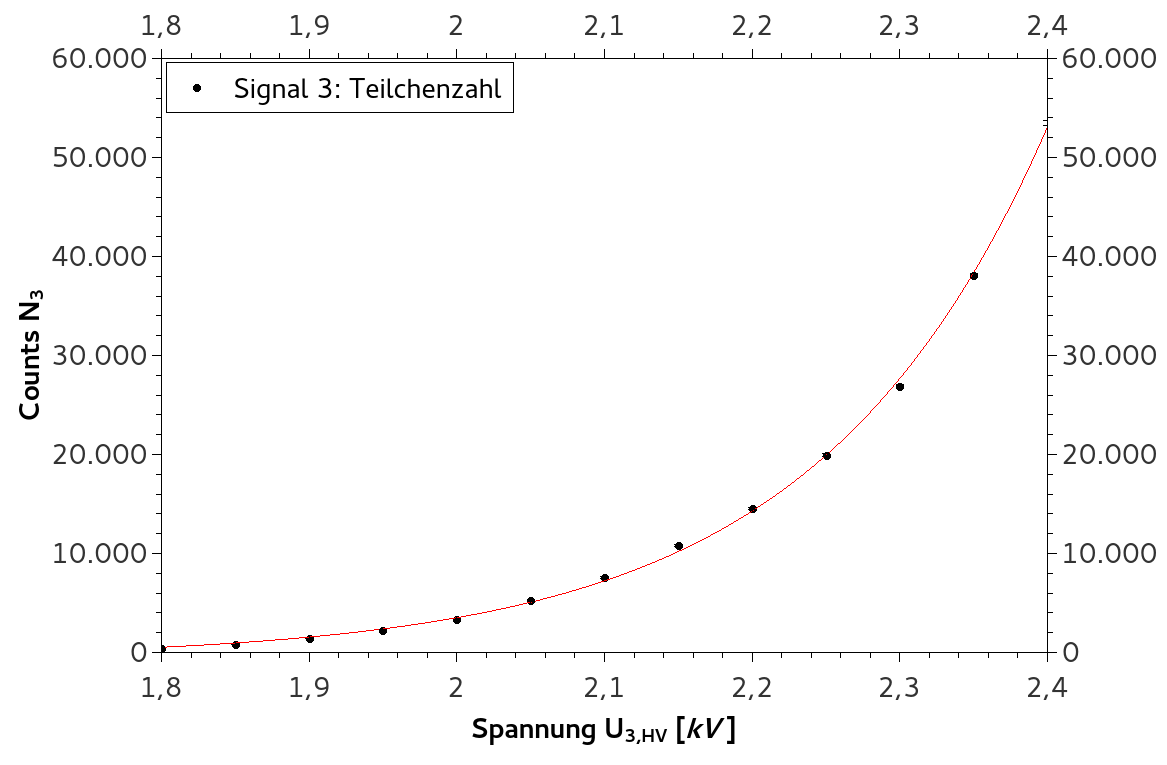
\includegraphics[scale=0.225]{pic/n3u3th}}
                \caption{Kennlinien der Hochspannung $U_{3,HV}$}
            \end{figure}
            Die Abbildungen \ref{n123} und \ref{n3} sehen sehr verschieden aus. Es ist stark auffällig, dass es sich bei \ref{n3} um ein exponentielles Wachstum handelt, während sich in \ref{n123} ein Plateau herausbildet, dessen verhalten eher einer kummulativen Verteilungsfunktion der Gauß-Kurve ähneln. 
            Die Unterschiede rühren vorallem daher, dass in \ref{n123} eine Triplezählrate vorliegt, für die Signale von allen Photomultipliern notwendig sind, um einen Count zu zählen. Es werden nur Signale gezählt, die in das Koinzidenzzeitfenster fallen und den Detektor in einer bestimmten, oben genannten Reihenfolge durchlaufen. In \ref{n3} handelt es sich um eine Singlezählrate, die nur den Photomultiplier 3 misst, dessen Hochspannung man verändert. Es wird kein Koinzidenzzeitfenster beachtet und es werden alle ankommenden Signale, bis auf das Signalrauschen, welches durch einen Diskriminator herausgefiltert wird, gemessen. Mit den steigenden Spannungen werden aus den im PM verbauten Dynoden mehr Elektronen herausgeschlagen. Damit steigt die Vervielfachung erheblich.\\
            Aus \ref{n123} kann man die Schwellspannung $U_{3,Schwell} = 2250\unit{V}$ ablesen. Sie wird als Optimierungsparamter im Hauptversuch benötigt.
        \subsubsection{Messung von Myon-Pulsen}
    \subsection{Hauptversuch}
        Für diesen Versuchsteil benötigt man die Schwellspannungen der einzelnen Photomultiplier. $$ U_{1,Schwell} = 2400\unit{V};\ U_{2,Schwell} = 2400\unit{V};\ U_{3,Schwell} = 2250\unit{V} $$. Die Schwellspannung von PM1 und PM2 wurden von Gruppe A ermittelt und an alle Gruppen weitergegeben. Sie sind durch Ablesen von den Kennlinien-Diagrammen (vgl. Abb. \ref{n123}) mit Fehlern behaftet, die das Experiment nachhaltig beeinflussen können.
        Interessant sind die Diskriminatorspannungen $U_{n,D}$ der PM, da sie das Signalrauschen unterdrücken sollen. Sie liegen bei: $$ U_{1,D} = 200\unit{mV};\ U_{2,D} = 200,5\unit{mV};\ U_{3,D} = 200,6\unit{mV} $$
        Die Messdauer beträgt 5 Tage, das heißt $t_{Mess} = 5\cdot24\cdot60\cdot60\unit{s} = 432000\unit{s}$		% Durchführung
\section{Auswertung}
	Im Folgenden sei $\{N_{Kmin},\dots,N_{Kmax}\}$ die Menge der gemessenen Zählraten in den Kanälen $K_{min}$ bis $ K_{max}$. Es werden zum direkten Vergleich aller drei Methoden der Lebensdauerbestimmung die Kanäle $K = 20, \dots ,175$ verwendet. Hierbei hat jeder Kanal die Breite $\Delta t = 1/24\ \unit{\mu s}$ und es gibt kein Offset, wodurch sich die Kanalkalibrierung sehr einfach zu $\tau_K = K\cdot \Delta t$ ergibt. Die maximal messbare Zeit wird mit $T := t_{Kmax} = 7,292\ \unit{\mu s}$ bezeichnet. 
	\subsection{Exponentielles Zerfallsgesetz}
	Es wird nun ausgehend von der Stichprobe der $N = 39142$ gemessenen Lebensdauern $\{t_1,\dots,t_N\}$ ein \textit{Maximum-Likelihood-Schätzwert} für die mittlere Lebensdauer der Myonen $\hat{\tau}$ ermittelt werden. Ausgangspunkt dafür ist ein auf maximal $T$ beschränktes exponentielles Zerfallsgesetz mit der parameterabhängigen Wahrscheinlichkeitsdichte:
		\begin{equation}
			P(t_i|\tau) = \frac{1}{\tau}\cdot e^{-\frac{t_i}{\tau}} \cdot\frac{1}{1-e^{-\frac{\tau}{t_i}}}
		\end{equation}
	Zentrales Hilfsmittel zur Parameterschätzung ist die \textit{Likelihood-Funktion}, welche sich aufgrund der als statistisch unabhängig angenommenen Messungen als faktorisierte Wahrscheinlichkeitsdichte ergibt, in der Zufallsvariable und Schätzparameter die Rollen tauschen:
		\begin{equation}
			L(\tau|x_1,\dots,x_N) := \prod_{i = 1}^{N} P(t_i|\tau) 
		\end{equation}
	Diese gilt es nun zu maximieren. Da die Logarithmusfunktion auf ihrem gesamten Definitionsbereich streng monoton wachsend ist, ist es praktikabel die logarithmierte Likelihoodfunktion zu betrachten:
		\begin{equation} \label{eq:maxLH}
			0 \overset{!}{=} \frac{\mathrm{d}\ln L}{\mathrm{d} \tau}\bigg|_{\tau = \hat{\tau}}  
		\end{equation}
	Gleichung (\ref{eq:maxLH}) ergibt in unserem speziellen Fall eine implizite Gleichung für $\hat{\tau}$, welche sich mit den Setzungen $x := \hat{\tau}/T$ und $a_K := t_K/(T\cdot N)$ in der einheitenlosen Form (\ref{eq:mastereq}) darstellen lässt. Da tatsächlich keine Zeiten, sondern Zählraten in Kanälen gemessen werden, setzt man weiterhin $t_K = N_K \cdot \tau_K$.
		\begin{equation} \label{eq:mastereq}
					f(x|a_{Kmin},\dots,a_{Kmax}) := \sum_{K = K_{min}}^{K_{max}} a_K(N_K,\tau_K,N,T) + \frac{1}{1 + e^{\frac{1}{x}}} - x \overset{!}{=} 0  
		\end{equation}
	Somit muss nur noch die Nullstelle dieser Funktion $f$ bestimmt werden, um den Schätzwert zu erhalten. Da $f$ offenbar stetig differenzierbar ist, erweist sich das \textit{Newton-Verfahren} als sinnvolle Methode zur Nullstellenapproximation. Hierbei wird ausgehend von einem Startwert $x_0$, welcher nicht zu weit von der Nullstelle entfernt sein sollte, eine Linearisierung von $f$ vorgenommen und die Nullstelle der so gewonnenen Tangente als bessere Näherung für den gesuchten Nulldurchgang $a$ verwendet. Die $(n+1)$-te Iteration ergibt sich rekursiv zu:
		\begin{equation} 
			x_{n+1} := x_n - \frac{f(x_n)}{f'(x_n)}
		\end{equation}
	Da sich für alle $n\in \mathbb{N}$ und eine Konstante $\alpha\in \mathbb{R}$ die Abschätzung:
		 \begin{equation} 
		 			\alpha \abs{x_{n}-a}\leq (\alpha \abs{x_{n-1}-a})^2\leq \dots \leq (\alpha\abs{x_0-a})^{2^n}
		 \end{equation}
	ergibt, konvergiert dieses Verfahren im Idealfall \textit{quadratisch} gegen $a$, d.h. in jedem Schritt verdoppelt sich die Anzahl an korrekten Dezimalstellen. Somit findet man einen hinreichend exakt approximierten Schätzwert $a = \hat{\tau}/T$ innerhalb weniger Iterationen. Da, wie sich herausstellte, die Lösung dieser Gleichung stark von der Wahl der verwendeten Kanäle abhängig ist, werden im Folgenden die Resultate zweier Kanalkonstellationen in Tabelle \ref{table:resExp}  zusammengestellt.\\
		\begin{table}[hp]
			\centering
			\begin{tabular}{c|c|c|c|c} 
				$K_{min}$		&		$K_{max}$		&		$T/\mu s$		&		$a = \hat{\tau}/T$		&		$\hat{\tau}/\mu s$\\
				\hline
				$20$			&		$175$			&		$7,292$			&		$0,598 \pm 0,004$		&		$4,36 \pm 0,03$\\	
				$11$			&		$200$			&		$8,333$			&		$0,260 \pm 0,002$		&		$2,17 \pm 0,02$		
			\end{tabular}
			\caption{Ermittelte Schätzwerte für unterschiedliche Messkanäle.}
			\label{table:resExp} 
		\end{table}
	\ \\
	Hierbei wurde mittels Fehlerfortpflanzung die Standardabweichung unter Ausnutzung der poissonverteilten Zählraten $\sigma_{Ni} = \sqrt{N_i}$ wie folgt bestimmt:
		\begin{equation} 
			\sigma_{\hat{\tau}} = \frac{1}{N}\sqrt{\sum\nolimits_{K=K_{min}}^{K_{max}} N_K\cdot \tau_K^2}
		\end{equation}	
	Die Abbildungen \ref{fig:LDexpZerf1} und \ref{fig:LDexpZerf2} visualisieren die graphische Lösung der impliziten Gleichung (\ref{eq:mastereq}). Die starke Abhängigkeit von den verwendeten Kanälen erklärt sich erst bei genauerem betrachten der Messdaten. Es stellt sich heraus, dass die Zählraten in den Kanälen 3 bis 15  mit einer Größenordnung $\mathcal{O}(10^3)$ zehnfach so groß sind, wie jene in den 'erwarteten Kanälen' (ab 40). Dies könnte durch zufällige Koinzidenzen ausgelöst werden, welche zum Beispiel durch Reaktion der Szintillatoren auf die uns natürlich umgebende Radioaktivität verursacht werden können. Man sieht, dass der ermittelte Schätzwert der Kanäle 11 bis 200 nahezu mit dem Literaturwert (\ref{eq:lit}) übereinstimmt, während die leicht verschobene Vergleichskonstellation um den Faktor 2 zu groß ist. Diese starke Abhängigkeit von den Kanälen soll durch Berücksichtigung des gebinnten Charakters der Messwerte in den nächsten beiden Kapiteln beseitigt werden. \\
		\begin{figure}[Hp]
		    \centering
		    \captionsetup{justification=centering}
		    \includegraphics[width=1.\linewidth]{pic/expZerf.pdf}
			\caption{Ermittlung der Lebensdauer durch Bestimmung der Nullstelle von $f$ (grüner Punkt) wobei die Kanäle 17 bis 175 genutzt worden.}
			\label{fig:LDexpZerf1}
		\end{figure}	
		
		\begin{figure}[Hp]
			\centering
			\captionsetup{justification=centering}
		    \includegraphics[width=1.\linewidth]{pic/expZerf2.pdf}
		    \caption{Ermittlung der Lebensdauer durch Bestimmung der Nullstelle von $f$ (grüner Punkt) wobei die Kanäle 11 bis 200 genutzt worden.}
		    \label{fig:LDexpZerf2}
		\end{figure}
			
	\subsection{Poissonverteilung}\label{sec:poisson}
		Im Folgenden behandeln wir die Verteilung der gemessenen Zählraten als eine \textit{Poissonverteilung}, was unter Anbetracht der großen Zahl an Kanälen eine sinnvolle Annahme ist. Die Zählratenverteilung im $K$-ten Kanal wird durch den charakteristischen Parameter des Erwartungswertes $\lambda_K$ beschrieben. Erwartet man bei einem festen $\tau$ $\lambda_K(\tau)$ Einträge im Zeitkanal $K$, so wird die Wahrscheinlichkeit, tatsächlich $N_K$ Ereignisse gemessen zu haben beschrieben durch:
			\begin{equation} \label{eq:poisson}
				P(N_K|\lambda_K(\tau)) = \frac{\lambda_K^{N_K}}{N_K!}e^{-\lambda_K}
			\end{equation}
		Es werden nun diskrete gebinnte Zeiten $(t_K, t_K + \Delta t)$ mit $\Delta t = 1/24\ \unit{\mu s}$ und $K = K_{min},\dots,K_{max}$ zugelassen. Da die Verteilung in den einzelnen Kanälen immer noch mit einem exponentiellen Zerfallsgesetz beschrieben wird, in diesem Fall aber nicht über alle Zeiten $t_K$ integriert wird, ergibt sich eine von $\tau$ abhängige Normierungskonstante $N_0$.
			\begin{equation}\label{eq:lamdbda}
				\lambda_K(\tau,N_0(\tau)|t_K,\Delta t) \approx N_0(\tau)\cdot \frac{\Delta t}{\tau} \cdot e^{-(t_K+\Delta t/2)/\tau}
			\end{equation} 
			\begin{equation}
				N_0(\tau) = \frac{N}{e^{-t_{Kmin}/\tau}-e^{-(t_{Kmax}+\Delta t)/\tau}}	
			\end{equation} 
			\begin{equation}\label{eq:N}
				N = \sum_{K = K_{min}}^{K_{max}} N_K	
			\end{equation} 
		Die Anwendung des Maximum-Likelihood-Kalküls auf die Verteilung (\ref{eq:poisson}) führt auf die Minimierung der effektiven Likelihood-Funktion $-2\ln L$. in dieser Darstellung ist es besonders leicht, die Standardabweichung $\sigma_{\hat{\tau}}$ abzulesen. Dafür ermittelt man die Stelle, in der $-2 \ln L$ um eine Einheit gegenüber dem Minimum angestiegen ist. Daraus ergibt sich ein Minimierungsproblem für den einzigen Summanden der effektiven Likelihood-Funktion, der von $\tau$ abhängt:
			\begin{align}
				L_{\text{eff}}(\tau|N_{Kmin},\dots,N_{Kmax}) &:=  \sum_{K = K_{min}}^{K_{max}} -2 N_K \ln\lambda_K(\tau, N_0(\tau)|t_K,\Delta t)	
			\end{align} 
		Es wurden um einen Vergleich zur obigen Methode zu erhalten, die Kanäle $K_{min} = 20$ bis $K_{max} = 175$ verwendet. Abbildung \ref{fig:LDpoisson} zeigt das Ergebnis, welches bereits besser zu dem Literaturwert passt und zudem nur wenig von den verwendeten Kanälen abhängt.
		\begin{figure}[hp]
		      			\centering
		      			\captionsetup{justification=centering}
		      			\includegraphics[width=1.\linewidth]{pic/poisson.pdf}
		      			\caption{Ermittlung der Lebensdauer durch Bestimmung des Minimums (grüner Punkt) der effektiven Likelihoodfunktion mit zugrundeliegender Poissonverteilung.}
		      			\label{fig:LDpoisson}
		\end{figure}
   \subsection{Normalverteilung}	
   Da die Poissonverteilung im Grenzfall $\lambda_K \gg 1$ in die \textit{Normalverteilung} übergehen sollte, werden nun jeweils benachbarte Kanäle zu einem zusammengefasst, sodass die Zählraten hinreichend groß sind. Nutzt man den arithmetischen Mittelwert der beiden Kanalmitten als neue Lebensdauer ergibt sich eine leicht kompliziertere Kanalkalibrierung:
   		\begin{equation}
   				\tau_K = K \cdot \Delta t - \frac{1}{48}\ \unit{\mu s}	
   		\end{equation} 
   Hierbei ist die neue Kanalbreite $\Delta t = 1/12\ \unit{\mu s}$. Die Wahrscheinlichkeitsdichtefunktion, die die Verteilung der im $K$-ten Kanal tatsächlich gemessenen Zählrate beschreibt, ergibt sich zu:
   		\begin{equation}
      			P(N_K|\mu_K(\tau),\sigma_K(\tau)) = \frac{1}{\sqrt{2\pi\sigma_K^2}}e^{-\frac{1}{2}\left(\frac{N_K- \mu_K}{\sigma_K}\right)^2}	
      	\end{equation} 
    Mit der Setzung $\mu_K = \lambda_K$ erhält man die gleichen Parameter wie in Abschnitt \ref{sec:poisson} in den Gleichungen (\ref{eq:lamdbda}) - (\ref{eq:N}). Für die Standardabweichung behält man die charakteristische Breite der Poissonverteilung $\sigma_K = \sqrt{\mu_K} \approx\sqrt{N_K}$.
    Es ergibt sich erneut ein Minimierungsproblem für $-2\ln L$. Der einzige Term, der von $\tau$ abhängt und der somit graphisch minimiert werden muss, ist:
    	\begin{equation}
          	\chi^2(\tau|N_{Kmin},\dots,K_{Kmax}) := \sum_{K = K_{min}}^{K_{max}} \left(\frac{N_K - \mu_K(\tau)}{\sigma_K}\right)^2	
         \end{equation}
    Die Standardabweichung kann erneut leicht abgelesen werden, indem man sich um eine Einheit vom Minimum von $\chi^2$ wegbewegt. Dies kann damit erklärt werden, da $\chi^2$ bis auf einen Faktor $-1/2$ dem Exponenten der Gaußverteilung entspricht, mit dem die Verteilung von $\tau$ beschrieben wird. Da die Normalverteilung $N(\tau|\mu,\sigma)$ an ihren Wendepunkten $\tau = \mu \pm \sigma$ gerade um einen Faktor $1/\sqrt{e}$ abgefallen ist, ist die Funktion $-2 \ln N$ gerade um eine Einheit gegenüber dem Minimum gestiegen:
    	\begin{equation}
    	       \tilde{N}(\tau) := -2 \ln N(\tau) = \ln(2\pi\sigma^2)  + \left(\frac{\tau - \mu}{\sigma}\right)^2 \equiv \tilde{N}(\tau = \mu) + \tilde{\chi}^2(\tau)	
    	\end{equation}
    	\begin{equation}
    	    	\tilde{N}(\tau = \mu \pm \sigma) - \tilde{N}(\tau = \mu) = \tilde{\chi}^2(\tau = \mu \pm \sigma) = 1 	
    	 \end{equation}
    Somit ist $\chi^2$ ein Maß für den Abfall der Gaußfunktion bezüglich des Maximums und ist im Wendepunkt genau 1. Abbildung \ref{fig:LDgauss} zeigt  das Ergebnis des Minimierungsproblems für die Kanäle $K_{min} = 20$ bis $K_{max} = 175$, sowie einen Vergleich zur Lösung des Problems ohne vorher die Kanäle zusammenzufassen. Es fällt auf, sich die Likelihood-Funktion zwar verändert, der Schätzwert allerdings fast unverändert ist. Das ist ein Anzeichen dafür, dass bereits vor dem Zusammenfassen der Kanäle die Näherungsbedingung $\lambda_K \gg 1$ hinreichend gut erfüllt war. Weiterhin wurde der in Abschnitt \ref{sec:poisson} ermittelte Wert nur wenig nach unten korrigiert. Da dieses Verfahren auch weniger sensitiv auf die Kanalauswahl reagiert, kann man auch dieses Ergebnis als vertrauenswürdig erachten.
   		\begin{figure}[hp]
      		   			\centering
      		   			\captionsetup{justification=centering}
      		   			\includegraphics[width=1.\linewidth]{pic/gauss.pdf}
      		   			\caption{Ermittlung der Lebensdauer durch Bestimmung des Minimums von $\chi^2(\tau)$. blauer Graph: $\chi^2$ mit zusammengefassten Kanälen, grüner Graph: ohne diese zusammenzufassen.}
      		   			\label{fig:LDgauss}	
      	\end{figure}
    
      		
      					% Auswertung
%\section{Zusammenfassung und Diskussion}

\newpage
\section{Anhang}
In diesem Abschnitt findet sich das handschriftlich erstellte Messprotokoll mit der uns gegebenen Aufgabenstellung.\\
\begin{figure}[htbp]
    \subfigure[Aufgabenstellung]{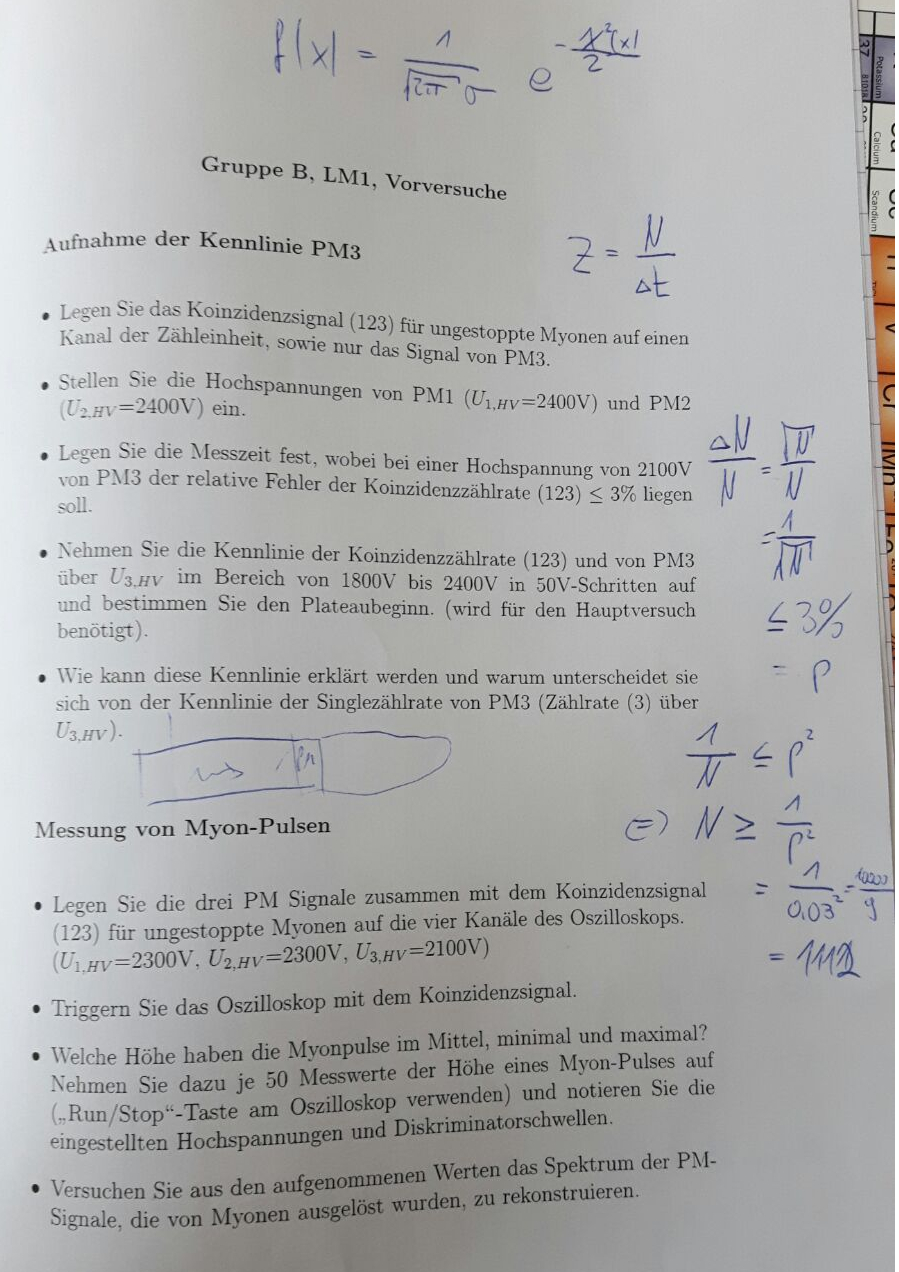
\includegraphics[scale=0.6]{pic/aufgabe.jpg}}
    \subfigure[S1, handschrftl. MP]{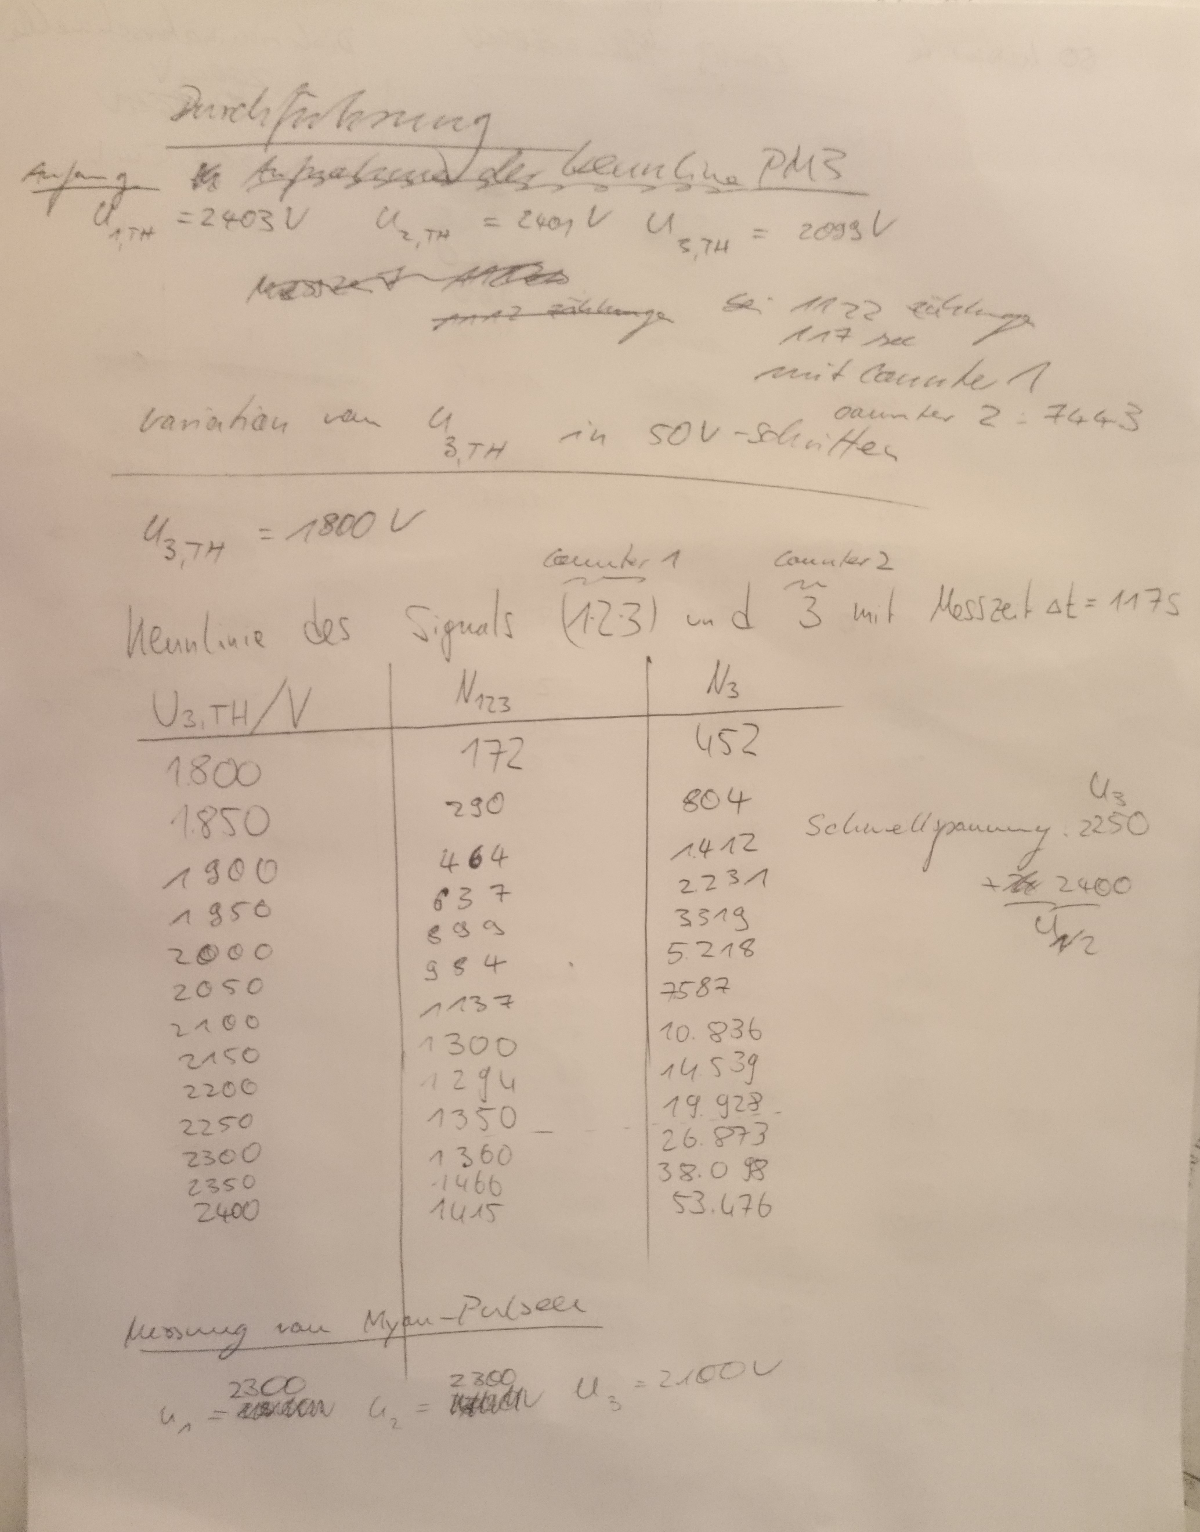
\includegraphics[scale=0.12]{pic/mess1.png}}
    \centering \subfigure[S2, handschiftl. MP]{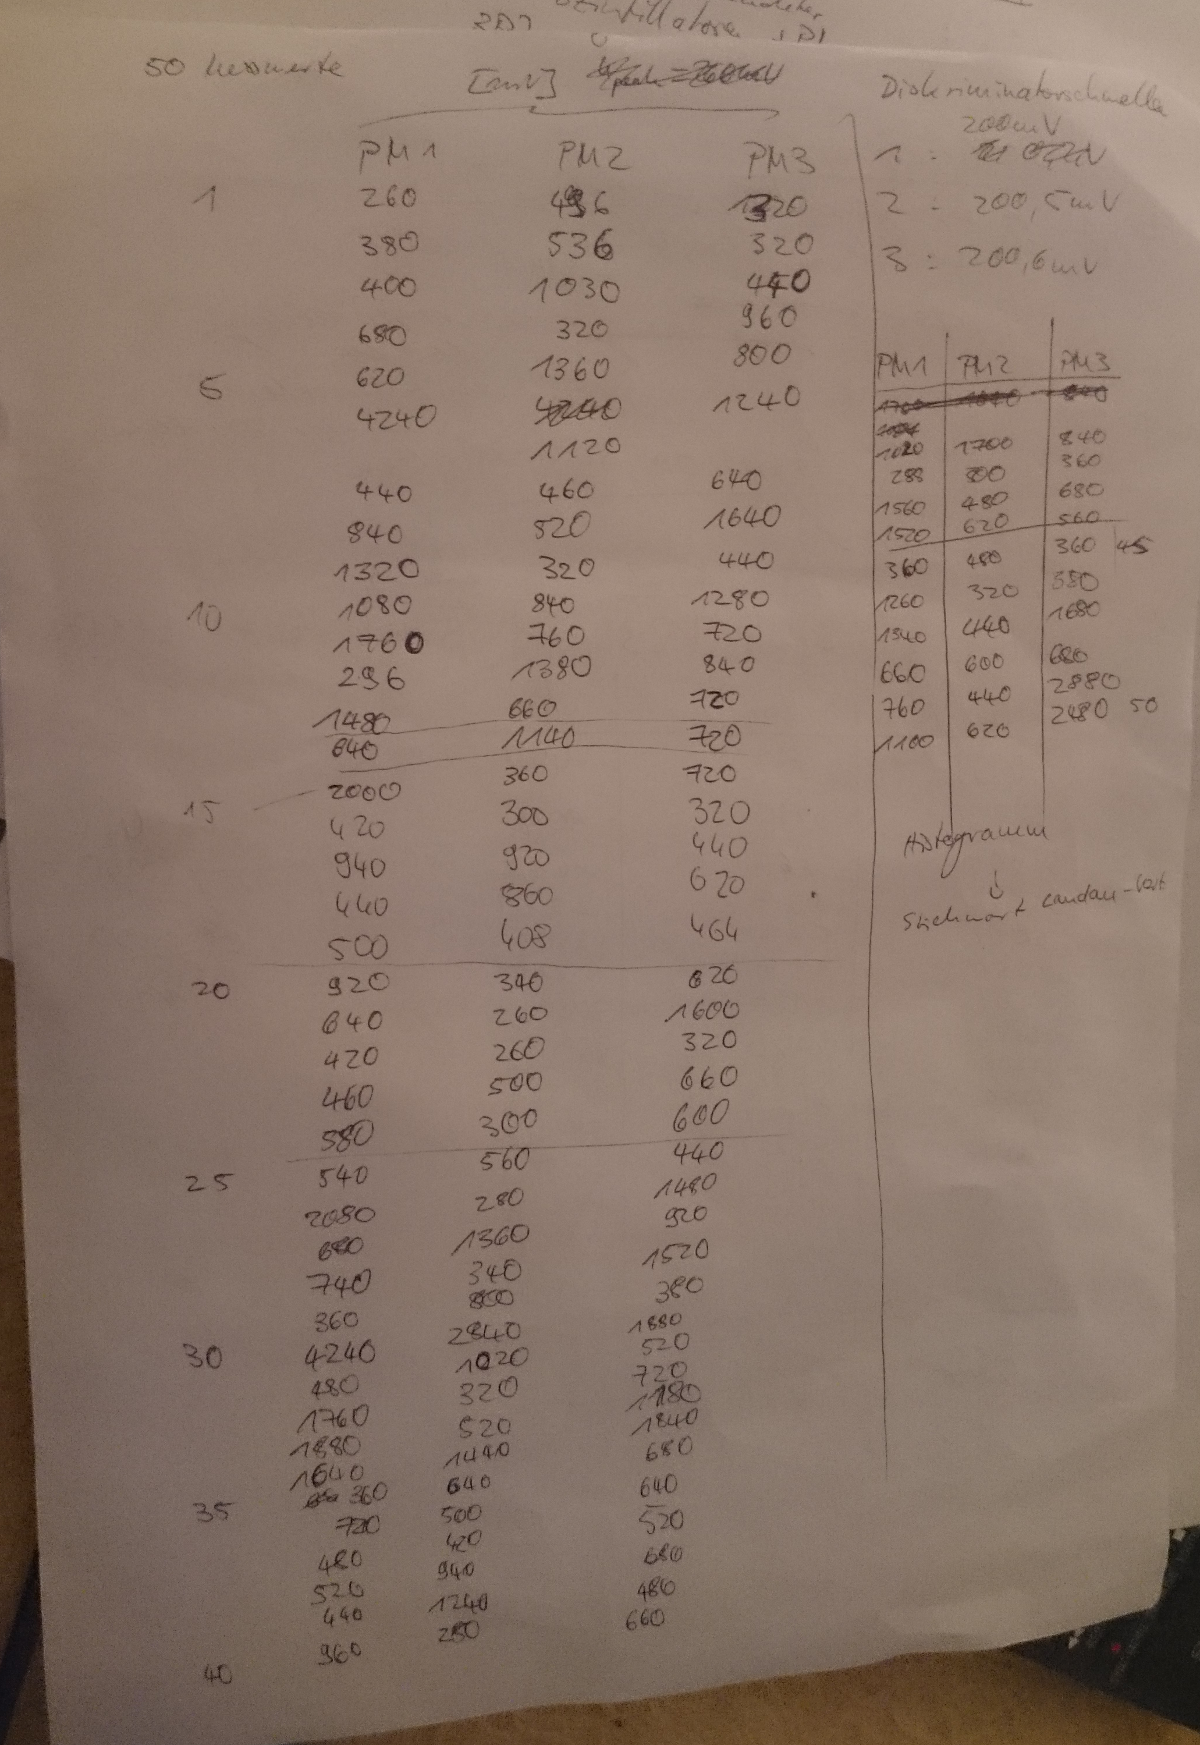
\includegraphics[scale=0.10]{pic/mess2.png}}
    \caption{Messprotokollseiten}
\end{figure}		% Diskussion
\begin{thebibliography}{99}
\bibitem [01] {PA} Technische Universität Dresden,  Institut für Kern- und Teilchenphysik: \textit{Lebensdauer von Myonen - Platzanleitung}. Dresden
\bibitem [02] {pdg} K.A Olive et al. (Particle Data Group), Chin. Phys. C, 38, 090001 (2014) and 2015 update.
\end{thebibliography}



\end{document}
